% --- ARQUIVO COMPLETO: 1-introducao.tex (VERSÃO FINAL CORRIGIDA) ---

\begin{frame}
\frametitle{Sumário}
\tableofcontents
\end{frame}

\section{Introdução e Definição do Problema}

% SLIDE 2: O GANCHO
\begin{frame}
\frametitle{Qual é o melhor caminho?}
\begin{columns}[T,onlytextwidth]
    \begin{column}{0.6\textwidth}
        \begin{block}{A Pergunta Intuitiva}
        Como o Google Maps sabe a rota mais rápida para chegar na FCT?
        \end{block}
        \begin{itemize}
            \item É o caminho mais rápido (menor tempo)?
            \item É o caminho mais curto (menor distância)?
            \item É o caminho mais barato (sem pedágios)?
        \end{itemize}
        \vspace{0.5cm}
        A ideia central é modelar o mapa como um \textbf{grafo} e atribuir \textbf{custos} às ruas.
    \end{column}
    \begin{column}{0.4\textwidth}
        \centering
        \includegraphics[width=\linewidth]{images/googlemaps.png}
    \end{column}
\end{columns}
\end{frame}

% SLIDE 3: APLICAÇÕES PRÁTICAS
\begin{frame}
\frametitle{Onde encontrar o PCM}
\begin{itemize}
    \item \textbf{Redes de Computadores:} Roteamento de pacotes na internet (Protocolo OSPF) — o custo é a latência.
    \item \textbf{Logística e Transporte:} Otimização de rotas de entrega (Correios, Mercado Livre) — o custo é a distância ou tempo.
    \item \textbf{Finanças (Avançado):} Detecção de oportunidades de arbitragem em mercados (encontrar ciclos de custo negativo).
    \item \textbf{Análise de Redes Sociais:} Medir o "grau de separação" entre duas pessoas.
\end{itemize}
\end{frame}

% SLIDE 4: DEFINIÇÃO FORMAL - PARTE 1
\begin{frame}
\frametitle{Traduzindo o Mapa para a Matemática}
\begin{columns}[T,onlytextwidth]
    \begin{column}{0.6\textwidth}
        \begin{itemize}
            \item \textbf{Grafo (ou Dígrafo):} $G = (V, E)$
            \item \textbf{$V$ (Vértices):} O conjunto de "nós" (ex: cidades, roteadores).
            \item \textbf{$E$ (Arestas):} O conjunto de "conexões" (ex: ruas, cabos).
            \item \textbf{Grafo Ponderado:} Cada aresta $(i, j) \in E$ possui um \textbf{peso} (ou custo) $w_{ij}$ associado.
        \end{itemize}
    \end{column}
    \begin{column}{0.4\textwidth}
        \centering
        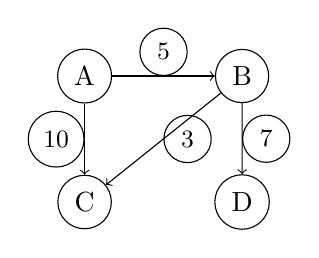
\begin{tikzpicture}[scale=0.8, every node/.style={circle, draw, minimum size=0.6cm}]
            \node (A) at (0,0) {A};
            \node (B) at (2.5,0) {B};
            \node (C) at (0,-2) {C};
            \node (D) at (2.5,-2) {D};
            \draw[->] (A) -- node[above, font=\small]{5} (B);
            \draw[->] (A) -- node[left, font=\small]{10} (C);
            \draw[->] (B) -- node[right, font=\small]{3} (C);
            \draw[->] (B) -- node[right, font=\small]{7} (D);
        \end{tikzpicture}
    \end{column}
\end{columns}
\end{frame}

\begin{frame}
\frametitle{O Problema de Caminhos Mínimos}
\begin{itemize}
    \item \textbf{Caminho:} Uma sequência de arestas que conecta um nó origem $s$ a um nó destino $t$.
    \begin{itemize}
        \item Ex: $P = (A \to B \to D)$
    \end{itemize}
    \item \textbf{Custo do Caminho:} A soma dos pesos $w_{ij}$ das arestas que formam o caminho.
    \begin{itemize}
        \item Ex: $Custo(P) = w_{AB} + w_{BD}$
    \end{itemize}
\end{itemize}

\vspace{0.3cm}
\begin{exampleblock}{Intuição}
    Queremos encontrar o caminho mais “barato” ou “curto” entre dois pontos em um grafo.
\end{exampleblock}
\end{frame}

\begin{frame}
\frametitle{Formulação Matemática do Problema}
\begin{block}{O Grande Objetivo}
    Dado um grafo ponderado $G$, um nó origem $s$ e um nó destino $t$, encontrar o caminho $P$ de $s$ para $t$ que \textbf{minimiza o custo total}.
    \[
      P^* = \arg\min_{P:\, s\to t} \sum_{(i,j)\in P} w_{ij}
    \]
\end{block}

\vspace{0.3cm}
\begin{alertblock}{Observação Importante}
    Os algoritmos que vamos estudar (Dijkstra, Bellman-Ford) resolvem o problema de \textbf{Origem Única (SSSP)}: encontram o caminho mínimo de $s$ para \textbf{TODOS} os outros nós.
\end{alertblock}
\end{frame}

% --- MÓDULO 2: MODELO MATEMÁTICO ---

\section{Modelo Matemático (PL)}

% SLIDE 6: A Abordagem Genérica
\begin{frame}
\frametitle{Modelo PL: A Abordagem Genérica}
\begin{itemize}
    \item \textbf{Ideia:} Modelar como um \textbf{Problema de Fluxo} para enviar 1 unidade da origem $s$ ao destino $t$.
\end{itemize}

\pause
\begin{block}{Variáveis de Decisão}
$x_{ij} = 
\begin{cases} 
1, & \text{se o arco } (i, j) \text{ for usado no caminho;} \\[4pt]
0, & \text{caso contrário.}
\end{cases}$
\end{block}

\pause
\begin{block}{Função Objetivo (Minimizar o Custo Total)}
Minimizar a soma dos custos de todas as arestas usadas:
\[
\min Z = \sum_{(i,j) \in E} w_{ij} \cdot x_{ij}
\]
\end{block}
\end{frame}

\begin{frame}
\frametitle{Modelo PL: Restrições de Conservação de Fluxo}
\begin{block}{Restrições}
\begin{itemize}
    \item \textbf{Origem ($s$):} Fluxo que \textbf{sai} = 1
    \[
    \sum_{j:(s,j)\in E} x_{sj} = 1
    \]
    \pause
    \item \textbf{Nós intermediários ($k$):} Fluxo que \textbf{entra} = Fluxo que \textbf{sai}
    \[
    \sum_{i:(i,k)\in E} x_{ik} - \sum_{j:(k,j)\in E} x_{kj} = 0
    \]
    \pause
    \item \textbf{Destino ($t$):} Fluxo que \textbf{entra} = 1
    \[
    \sum_{i:(i,t)\in E} x_{it} = 1
    \]
\end{itemize}
\end{block}
\end{frame}

% SLIDE 7: Exemplo de Modelagem (Grafo A-E)
\begin{frame}
\frametitle{Exemplo de Modelagem: Grafo Logístico}
\begin{itemize}
    \item Vamos modelar o problema de achar a rota de custo mínimo da Origem \textbf{A} para o Destino \textbf{E}.
\end{itemize}
\begin{columns}[T,onlytextwidth]
    \begin{column}{0.7\textwidth}
        \centering
        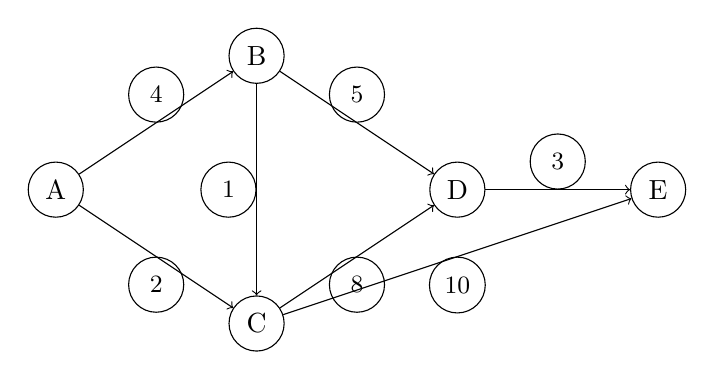
\begin{tikzpicture}[scale=0.85, every node/.style={circle, draw, minimum size=0.7cm}]
            \node (A) at (0, 2) {A};
            \node (B) at (3, 4) {B};
            \node (C) at (3, 0) {C};
            \node (D) at (6, 2) {D};
            \node (E) at (9, 2) {E};
            
            \draw[->] (A) -- node[above, font=\small]{4} (B);
            \draw[->] (A) -- node[below, font=\small]{2} (C);
            \draw[->] (B) -- node[left, font=\small]{1} (C);
            \draw[->] (B) -- node[above, font=\small]{5} (D);
            \draw[->] (C) -- node[below, font=\small]{8} (D);
            \draw[->] (C) -- node[below, font=\small]{10} (E);
            \draw[->] (D) -- node[above, font=\small]{3} (E);
        \end{tikzpicture}
    \end{column}
    \begin{column}{0.5\textwidth}
        \textbf{Custos ($w_{ij}$):}
        \begin{itemize}
            \item $w_{AB} = 4$
            \item $w_{AC} = 2$
            \item $w_{BC} = 1$
            \item $w_{BD} = 5$
            \item $w_{CD} = 8$
            \item $w_{CE} = 10$
            \item $w_{DE} = 3$
        \end{itemize}
    \end{column}
\end{columns}
\end{frame}

% SLIDE 8: O PPL Completo
\begin{frame}
\frametitle{Exemplo de Modelagem: O PPL Completo}

\textbf{Função Objetivo (Minimizar Z):}
\begin{tiny}
\[
\min Z = 4x_{AB} + 2x_{AC} + 1x_{BC} + 5x_{BD} + 8x_{CD} + 10x_{CE} + 3x_{DE}
\]
\end{tiny}

\textbf{Sujeito a (Conservação de Fluxo):}
\begin{scriptsize}
\begin{align*}
x_{AB} + x_{AC} &= 1 && \text{(Nó A: Origem)} \\
x_{BC} + x_{BD} - x_{AB} &= 0 && \text{(Nó B: Intermediário)} \\
x_{CD} + x_{CE} - x_{AC} - x_{BC} &= 0 && \text{(Nó C: Intermediário)} \\
x_{DE} - x_{BD} - x_{CD} &= 0 && \text{(Nó D: Intermediário)} \\
x_{CE} + x_{DE} &= 1 && \text{(Nó E: Destino)} \\
x_{ij} &\in \{0,1\}, \quad \forall (i,j)
\end{align*}
\end{scriptsize}

\textbf{Interpretação:} 
\begin{scriptsize}
Cada variável $x_{ij}$ indica se o arco $(i,j)$ faz parte do caminho mínimo (1) ou não (0).  
O modelo garante que o fluxo parte de A, passa por nós intermediários e chega em E com o menor custo total.
\end{scriptsize}

\end{frame}

\begin{frame}
\frametitle{Modelo PL: A Mágica da Integridade}

\begin{itemize}
    \item \textbf{Questão:} É necessário impor explicitamente que as variáveis $x_{ij}$ assumam apenas valores inteiros ($0$ ou $1$)?
    \[
    x_{ij} \in \{0, 1\} \quad \text{(Programação Inteira)}
    \]

    \item \textbf{Observação:} Para este tipo de problema de rede, a imposição de integralidade não é necessária.

    \item Modelos de \textbf{Fluxo de Custo Mínimo} — como o problema de caminho mínimo — possuem uma estrutura matricial denominada \textbf{Totalmente Unimodular}. 

    \item \textbf{Consequência:} Quando a matriz de coeficientes do sistema de restrições é totalmente unimodular e os termos do lado direito (ofertas e demandas) são inteiros, o \textbf{problema de Programação Linear relaxado} (isto é, considerando apenas $x_{ij} \ge 0$) apresenta uma \textbf{solução ótima inteira}.

    \item \textbf{Em síntese:} A propriedade de total unimodularidade garante a integridade natural da solução, tornando desnecessária a formulação explícita como um problema de programação inteira.
\end{itemize}

\end{frame}

% --- MÓDULO 3: MÉTODOS DE RESOLUÇÃO ---

\section{Métodos de Resolução}

% SLIDE 10: INTRODUÇÃO AOS ALGORITMOS
\begin{frame}
\frametitle{Módulo 3: Métodos de Resolução}
\begin{itemize}
    \item Embora o modelo de PL seja academicamente correto, ele não é a forma mais \textit{eficiente} de resolver o Problema de Caminhos Mínimos na prática.
    \item Na prática, usamos algoritmos especializados em grafos que são muito mais rápidos.
    \item Vamos focar em dois algoritmos fundamentais:
    \begin{enumerate}
        \item \textbf{Algoritmo de Dijkstra}
        \item \textbf{Algoritmo de Bellman-Ford}
    \end{enumerate}
\end{itemize}
\end{frame}

% SLIDE 11: ALGORITMO DE DIJKSTRA (CONCEITO)
\begin{frame}
\frametitle{Algoritmo de Dijkstra}
\begin{block}{O Conceito}
Uma abordagem "Gulosa" (Greedy). A cada passo, ele escolhe o caminho que \textit{parece} ser o melhor (o mais curto) e expande a partir dele.
\end{block}

\begin{alertblock}{Restrição Crítica}
O Algoritmo de Dijkstra \textbf{NÃO FUNCIONA} se o grafo tiver arestas com \textbf{pesos negativos}.
\end{alertblock}
\end{frame}

% --- SLIDES 12-17: Exercício de Dijkstra ---
\begin{frame}
\frametitle{Exercício: Algoritmo de Dijkstra (Inicialização)}

\begin{columns}[T,onlytextwidth]
    % --- Coluna do grafo ---
    \begin{column}{0.7\textwidth}
        \centering
        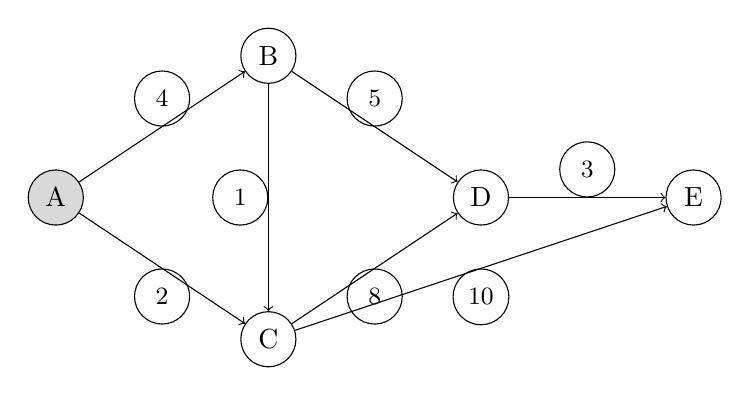
\begin{tikzpicture}[scale=0.9, every node/.style={circle, draw, minimum size=0.7cm}]
            \node[fill=gray!30] (A) at (0, 2) {A}; % Nó inicial
            \node (B) at (3, 4) {B};
            \node (C) at (3, 0) {C};
            \node (D) at (6, 2) {D};
            \node (E) at (9, 2) {E};
            
            \draw[->] (A) -- node[above, font=\small]{4} (B);
            \draw[->] (A) -- node[below, font=\small]{2} (C);
            \draw[->] (B) -- node[left, font=\small]{1} (C);
            \draw[->] (B) -- node[above, font=\small]{5} (D);
            \draw[->] (C) -- node[below, font=\small]{8} (D);
            \draw[->] (C) -- node[below, font=\small]{10} (E);
            \draw[->] (D) -- node[above, font=\small]{3} (E);
        \end{tikzpicture}
    \end{column}
    
    % --- Coluna da tabela ---
    \begin{column}{0.3\textwidth}
        \textbf{Nós Visitados: \{\}} \\[4pt]
        {\footnotesize
        \setlength{\tabcolsep}{6pt}
        \renewcommand{\arraystretch}{1.1}
        \begin{tabular}{c|c|c}
            \textbf{Nó} & \textbf{dist[i]} & \textbf{prev[i]} \\ \hline
            A & \textbf{0} & - \\
            B & $\infty$ & - \\
            C & $\infty$ & - \\
            D & $\infty$ & - \\
            E & $\infty$ & - \\
        \end{tabular}}
        \vspace{6pt}
        
        \textbf{Próximo nó:} A (custo 0)
    \end{column}
\end{columns}

\end{frame}

\begin{frame}
\frametitle{Exercício: Dijkstra - Iteração 1 (Nó A)}

\begin{columns}[T,onlytextwidth]
    % --- Coluna do grafo ---
    \begin{column}{0.58\textwidth}
        \centering
        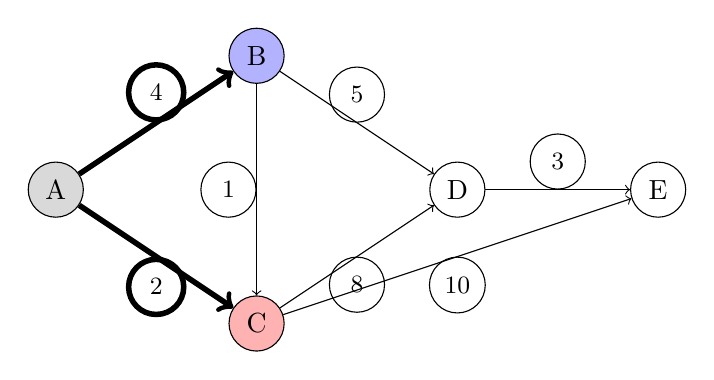
\begin{tikzpicture}[scale=0.85, every node/.style={circle, draw, minimum size=0.7cm}]
            \node[fill=gray!30] (A) at (0, 2) {A}; 
            \node[fill=blue!30] (B) at (3, 4) {B}; % Alcançado
            \node[fill=red!30] (C) at (3, 0) {C};  % Alcançado e menor
            \node (D) at (6, 2) {D};
            \node (E) at (9, 2) {E};
            
            \draw[->,line width=2pt] (A) -- node[above, font=\small]{4} (B); % Caminho usado
            \draw[->,line width=2pt] (A) -- node[below, font=\small]{2} (C); % Caminho usado
            \draw[->] (B) -- node[left, font=\small]{1} (C);
            \draw[->] (B) -- node[above, font=\small]{5} (D);
            \draw[->] (C) -- node[below, font=\small]{8} (D);
            \draw[->] (C) -- node[below, font=\small]{10} (E);
            \draw[->] (D) -- node[above, font=\small]{3} (E);
        \end{tikzpicture}
    \end{column}

    % --- Coluna da explicação e tabela ---
    \begin{column}{0.42\textwidth}
        \textbf{Visitando Nó: A} (dist = 0)
        \vspace{4pt}

        \begin{itemize}
            \item Vizinho B: $0 + 4 = 4$ → Atualiza dist[B]=4, prev[B]=A
            \item Vizinho C: $0 + 2 = 2$ → Atualiza dist[C]=2, prev[C]=A
        \end{itemize}

        \vspace{4pt}
        \textbf{Nós Visitados: \{A\}} \\[4pt]

        {\footnotesize
        \setlength{\tabcolsep}{6pt}
        \renewcommand{\arraystretch}{1.1}
        \begin{tabular}{c|c|c}
            \textbf{Nó} & \textbf{dist[i]} & \textbf{prev[i]} \\ \hline
            A & 0 & - \\
            B & \textbf{4} & A \\
            C & \textbf{2} & A \\
            D & $\infty$ & - \\
            E & $\infty$ & - \\
        \end{tabular}}

        \vspace{6pt}
        \textbf{Próximo nó:} C (menor dist = 2)
    \end{column}
\end{columns}

\end{frame}

\begin{frame}
\frametitle{Exercício: Dijkstra - Iteração 2 (Nó C)}

\begin{columns}[T,onlytextwidth]
    % --- Coluna do grafo ---
    \begin{column}{0.58\textwidth}
        \centering
        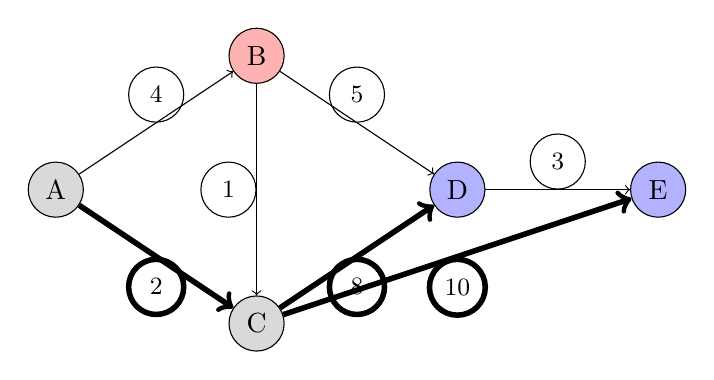
\begin{tikzpicture}[scale=0.85, every node/.style={circle, draw, minimum size=0.7cm}]
            \node[fill=gray!30] (A) at (0, 2) {A}; 
            \node[fill=red!30] (B) at (3, 4) {B}; % Menor
            \node[fill=gray!30] (C) at (3, 0) {C}; % Visitado
            \node[fill=blue!30] (D) at (6, 2) {D}; % Alcançado
            \node[fill=blue!30] (E) at (9, 2) {E}; % Alcançado
            
            \draw[->] (A) -- node[above, font=\small]{4} (B); 
            \draw[->,line width=2pt] (A) -- node[below, font=\small]{2} (C); % Caminho usado
            \draw[->] (B) -- node[left, font=\small]{1} (C);
            \draw[->] (B) -- node[above, font=\small]{5} (D);
            \draw[->,line width=2pt] (C) -- node[below, font=\small]{8} (D); % Caminho usado
            \draw[->,line width=2pt] (C) -- node[below, font=\small]{10} (E); % Caminho usado
            \draw[->] (D) -- node[above, font=\small]{3} (E);
        \end{tikzpicture}
    \end{column}

    % --- Coluna da explicação e tabela ---
    \begin{column}{0.42\textwidth}
        \textbf{Visitando Nó: C} (dist = 2)
        \vspace{4pt}

        \begin{itemize}
            \item Vizinho D: $2 + 8 = 10$ → Atualiza dist[D]=10, prev[D]=C
            \item Vizinho E: $2 + 10 = 12$ → Atualiza dist[E]=12, prev[E]=C
        \end{itemize}

        \vspace{4pt}
        \textbf{Nós Visitados: \{A, C\}} \\[4pt]

        {\footnotesize
        \setlength{\tabcolsep}{6pt}
        \renewcommand{\arraystretch}{1.1}
        \begin{tabular}{c|c|c}
            \textbf{Nó} & \textbf{dist[i]} & \textbf{prev[i]} \\ \hline
            A & 0 & - \\
            B & 4 & A \\
            C & 2 & A \\
            D & \textbf{10} & C \\
            E & \textbf{12} & C \\
        \end{tabular}}

        \vspace{6pt}
        \textbf{Próximo nó:} B (menor dist = 4)
    \end{column}
\end{columns}

\end{frame}

\begin{frame}
\frametitle{Exercício: Dijkstra - Iteração 3 (Nó B) - A "Relaxação"}

\begin{columns}[T,onlytextwidth]
    % --- Coluna do grafo ---
    \begin{column}{0.58\textwidth}
        \centering
        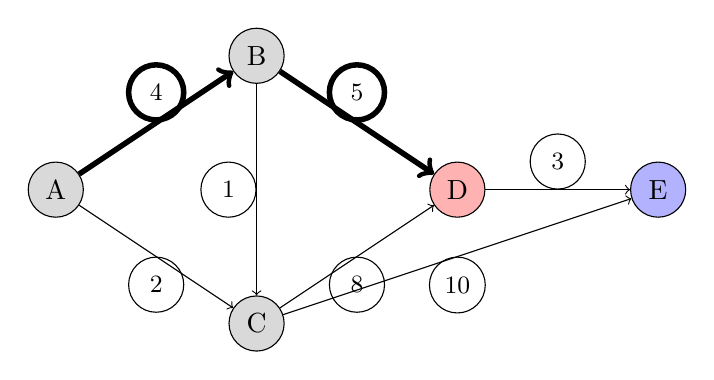
\begin{tikzpicture}[scale=0.85, every node/.style={circle, draw, minimum size=0.7cm}]
            \node[fill=gray!30] (A) at (0, 2) {A}; 
            \node[fill=gray!30] (B) at (3, 4) {B}; % Visitado
            \node[fill=gray!30] (C) at (3, 0) {C}; 
            \node[fill=red!30] (D) at (6, 2) {D}; % Menor
            \node[fill=blue!30] (E) at (9, 2) {E}; 
            
            \draw[->,line width=2pt] (A) -- node[above, font=\small]{4} (B); 
            \draw[->] (A) -- node[below, font=\small]{2} (C); 
            \draw[->] (B) -- node[left, font=\small]{1} (C);
            \draw[->,line width=2pt] (B) -- node[above, font=\small]{5} (D); % Caminho usado
            \draw[->] (C) -- node[below, font=\small]{8} (D);
            \draw[->] (C) -- node[below, font=\small]{10} (E);
            \draw[->] (D) -- node[above, font=\small]{3} (E);
        \end{tikzpicture}
    \end{column}

    % --- Coluna da explicação e tabela ---
    \begin{column}{0.42\textwidth}
        \textbf{Visitando Nó: B} (dist = 4)
        \vspace{4pt}

        \begin{itemize}
            \item Vizinho C: já visitado.
            \item Vizinho D: $4 + 5 = 9$.
            \item O custo atual de D é 10. \\[2pt]
                  \textbf{Como 9 < 10, atualizamos!}
            \item Atualiza dist[D] = 9, prev[D] = B
        \end{itemize}

        \vspace{4pt}
        \textbf{Nós Visitados: \{A, C, B\}} \\[4pt]

        {\footnotesize
        \setlength{\tabcolsep}{6pt}
        \renewcommand{\arraystretch}{1.1}
        \begin{tabular}{c|c|c}
            \textbf{Nó} & \textbf{dist[i]} & \textbf{prev[i]} \\ \hline
            A & 0 & - \\
            B & 4 & A \\
            C & 2 & A \\
            D & \textbf{9} & \textbf{B} \\
            E & 12 & C \\
        \end{tabular}}

        \vspace{6pt}
        \textbf{Próximo nó:} D (menor dist = 9)
    \end{column}
\end{columns}

\end{frame}


\begin{frame}
\frametitle{Exercício: Dijkstra - Iterações 4 e 5 (Nós D, E)}
\begin{columns}[T,onlytextwidth]
    \begin{column}{0.58\textwidth}
        \centering
        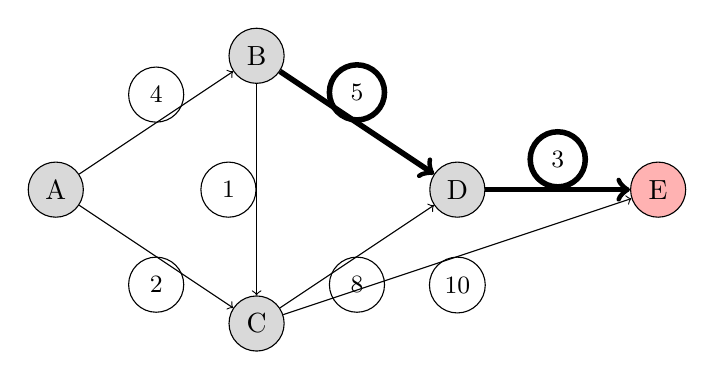
\begin{tikzpicture}[scale=0.85, every node/.style={circle, draw, minimum size=0.7cm}]
            \node[fill=gray!30] (A) at (0, 2) {A}; 
            \node[fill=gray!30] (B) at (3, 4) {B}; 
            \node[fill=gray!30] (C) at (3, 0) {C}; 
            \node[fill=gray!30] (D) at (6, 2) {D}; % Visitado
            \node[fill=red!30] (E) at (9, 2) {E}; % Menor
            
            \draw[->] (A) -- node[above, font=\small]{4} (B); 
            \draw[->] (A) -- node[below, font=\small]{2} (C); 
            \draw[->] (B) -- node[left, font=\small]{1} (C);
            \draw[->,line width=2pt] (B) -- node[above, font=\small]{5} (D); 
            \draw[->] (C) -- node[below, font=\small]{8} (D);
            \draw[->] (C) -- node[below, font=\small]{10} (E);
            \draw[->,line width=2pt] (D) -- node[above, font=\small]{3} (E); % Caminho usado
        \end{tikzpicture}
    \end{column}
    \begin{column}{0.42\textwidth}
        \textbf{Visitando Nó: D} (dist=9)
        \begin{itemize}
            \item Vizinho E: $9 + 3 = 12$.
            \item O custo atual de E é 12. Como $12 \not< 12$, \textbf{não há atualização}.
        \end{itemize}
        \textbf{Visitando Nó: E} (dist=12)
        \begin{itemize}
            \item Fim do algoritmo (destino alcançado / fila vazia).
        \end{itemize}
        
        \textbf{Nós Visitados: \{A, C, B, D, E\}}
        {\footnotesize\setlength{\tabcolsep}{6pt}\renewcommand{\arraystretch}{1.1}%
        \begin{tabular}{c|c|c}
        \textbf{Nó} & \textbf{dist[i]} & \textbf{prev[i]} \\ \hline
        A & 0 & - \\
        B & 4 & A \\
        C & 2 & A \\
        D & 9 & B \\
        E & 12 & C \\
        \end{tabular}}
    \end{column}
\end{columns}
\end{frame}

\begin{frame}
\frametitle{Exercício: Dijkstra — Conclusão e Caminho}

\begin{columns}[T,onlytextwidth]
    \begin{column}{0.45\textwidth}
        \begin{block}{Custos Mínimos a partir de A}
        \centering
        {\footnotesize
        \renewcommand{\arraystretch}{1.2}
        \begin{tabular}{c|c}
        \textbf{Nó} & \textbf{Custo (dist)} \\ \hline
        B & 4 \\
        C & 2 \\
        D & 9 \\
        E & 12 \\
        \end{tabular}
        }
        \end{block}
    \end{column}

    \begin{column}{0.55\textwidth}
        \begin{alertblock}{Caminho Mínimo (Backtracking)}
        \begin{itemize}
            \item \textbf{E} $\leftarrow$ C  
            \item \textbf{C} $\leftarrow$ A  
            \item Chegamos à origem: \textbf{A}
        \end{itemize}
        \vspace{0.2cm}
        \centering
        \textbf{Caminho:} $A \rightarrow C \rightarrow E$ \\[4pt]
        \textbf{Custo Total:} $2 + 10 = 12$
        \end{alertblock}
    \end{column}
\end{columns}
\end{frame}

\begin{frame}
\frametitle{Exercício: Algoritmo de Dijkstra (Inicialização)}

\begin{columns}[T,onlytextwidth]
    % --- Coluna do grafo ---
    \begin{column}{0.7\textwidth}
        \centering
        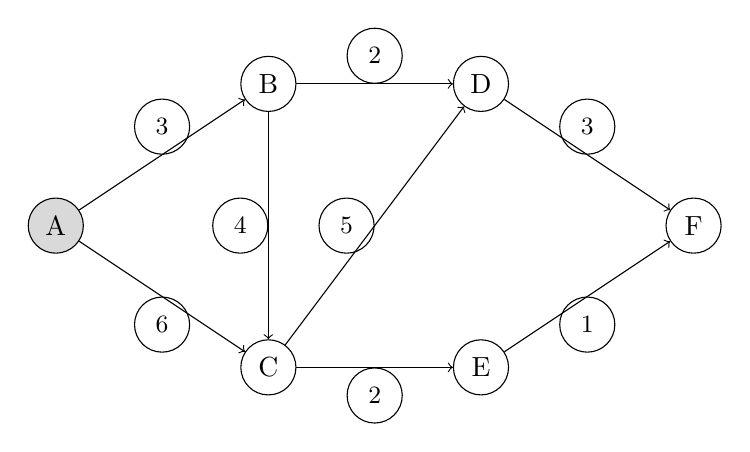
\begin{tikzpicture}[scale=0.9, every node/.style={circle, draw, minimum size=0.7cm}]
            % Nós
            \node[fill=gray!30] (A) at (0, 2) {A}; % Nó inicial
            \node (B) at (3, 4) {B};
            \node (C) at (3, 0) {C};
            \node (D) at (6, 4) {D};
            \node (E) at (6, 0) {E};
            \node (F) at (9, 2) {F};
            
            % Arestas
            \draw[->] (A) -- node[above, font=\small]{3} (B);
            \draw[->] (A) -- node[below, font=\small]{6} (C);
            \draw[->] (B) -- node[above, font=\small]{2} (D);
            \draw[->] (B) -- node[left, font=\small]{4} (C);
            \draw[->] (C) -- node[below, font=\small]{2} (E);
            \draw[->] (D) -- node[above, font=\small]{3} (F);
            \draw[->] (E) -- node[below, font=\small]{1} (F);
            \draw[->] (C) -- node[left, font=\small]{5} (D);
        \end{tikzpicture}
    \end{column}
    
    % --- Coluna da tabela ---
    \begin{column}{0.3\textwidth}
        \textbf{Nós Visitados: \{\}} \\[4pt]
        {\footnotesize
        \setlength{\tabcolsep}{6pt}
        \renewcommand{\arraystretch}{1.1}
        \begin{tabular}{c|c|c}
            \textbf{Nó} & \textbf{dist[i]} & \textbf{prev[i]} \\ \hline
            A & \textbf{0} & - \\
            B & $\infty$ & - \\
            C & $\infty$ & - \\
            D & $\infty$ & - \\
            E & $\infty$ & - \\
            F & $\infty$ & - \\
        \end{tabular}}
        \vspace{6pt}
        
        \textbf{Próximo nó:} A (custo 0)
    \end{column}
\end{columns}
\end{frame}

\begin{frame}
\frametitle{Algoritmo de Bellman-Ford}

\begin{block}{Ideia Geral}
O algoritmo de \textbf{Bellman-Ford} segue uma abordagem de \textbf{Programação Dinâmica}.
Diferente do Dijkstra, que é \textbf{guloso}, o Bellman-Ford é \textbf{cauteloso}: 
ele reavalia continuamente todas as arestas, garantindo o custo mínimo mesmo com pesos negativos.
\end{block}

\begin{alertblock}{Principais Vantagens}
\begin{itemize}
    \item \textbf{Funciona com pesos negativos.}
    \item \textbf{Detecta ciclos negativos}, isto é, caminhos que reduzem o custo infinitamente.
\end{itemize}
\end{alertblock}

\begin{block}{Ideia Principal}
Repete o processo de \textbf{relaxar todas as arestas} do grafo exatamente $|V|-1$ vezes,
onde $|V|$ é o número de vértices.
\end{block}
\end{frame}


\begin{frame}
\frametitle{Algoritmo de Bellman-Ford — Funcionamento}

\begin{block}{Por que repetir $|V|-1$ vezes?}
O maior caminho possível sem formar um ciclo contém, no máximo, $|V|-1$ arestas.
Após essas iterações, todos os menores caminhos já terão sido encontrados.
\end{block}

\begin{alertblock}{Detecção de Ciclos Negativos}
Após as $|V|-1$ passagens, o algoritmo faz uma \textbf{última verificação}:
\begin{itemize}
    \item Se ainda for possível “relaxar” alguma aresta, 
    significa que existe um \textbf{ciclo negativo}.
    \item Nesse caso, o algoritmo emite um alerta: \textbf{"Ciclo Negativo Detectado!"}
\end{itemize}
\end{alertblock}

\begin{exampleblock}{Aplicação Prática}
Em finanças, é usado para detectar \textbf{arbitragem}:
\textit{converter moedas em sequência (A → B → C → A) e terminar com lucro}.
\end{exampleblock}
\end{frame}


\begin{frame}
\frametitle{Comparativo: Dijkstra vs. Bellman-Ford}

\begin{table}[h!]
\centering
\renewcommand{\arraystretch}{1.2}
\begin{tabular}{|l|c|c|}
\hline
\textbf{Característica} & \textbf{Dijkstra} & \textbf{Bellman-Ford} \\ \hline
\textbf{Abordagem} & Gulosa (Greedy) & Programação Dinâmica \\ \hline
\textbf{Pesos Negativos} & x Não funciona & V Suportado \\ \hline
\textbf{Detecta Ciclos Negativos} & x Não & V Sim \\ \hline
\textbf{Complexidade} & $O(E \log V)$ ou $O(V^2)$ & $O(V \cdot E)$ \\ \hline
\textbf{Uso Típico} & Grafos sem pesos negativos & Grafos com pesos negativos \\ \hline
\textbf{Exemplo} & GPS, OSPF (redes) & Arbitragem financeira \\ \hline
\end{tabular}
\end{table}

\vspace{0.4cm}
\begin{block}{Conclusão}
\textbf{Dijkstra} é mais rápido e eficiente para grafos positivos.  
\textbf{Bellman-Ford}, embora mais lento, é mais \textbf{robusto e confiável} em cenários complexos.
\end{block}
\end{frame}

% --- MÓDULO 4: REFERÊNCIAS BIBLIOGRÁFICAS ---

\section{Referências Bibliográficas}

% Adiciona [allowframebreaks] para que o beamer possa
% dividir a lista em múltiplos slides se ela for muito longa
\begin{frame}[allowframebreaks]
\frametitle{Referências Bibliográficas}

% Adicione este comando para mostrar TODAS as referências do seu arquivo ref.bib
\nocite{*}

% Este comando puxa as referências do seu arquivo ref.bib
% e as formata usando o estilo ABNT (definido no panqueques.sty)
\printbibliography

\end{frame}